\begin{figure}
\centering
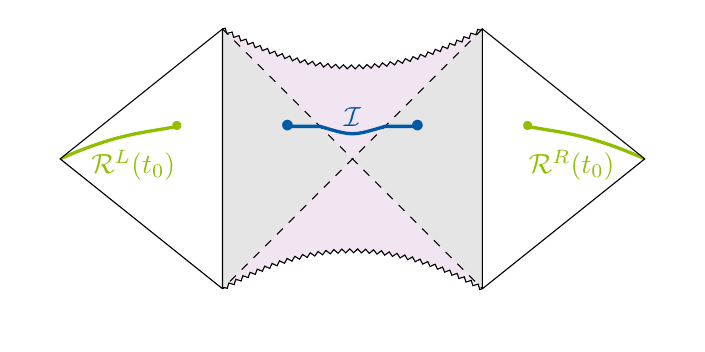
\begin{tikzpicture}[scale=1.65]
\node at (1.35,0.25) {\textcolor{black!25!lime}{\footnotesize$\bullet$}};
\draw[-,black!25!lime,very thick] (1.35,0.25)  .. controls (1.6,0.2) and (1.8,0.2) ..  (2.25,0);
\draw[-,draw=none,fill=white] (1,1) to (2.25,0) to (2.5,0) to (1.25,1) to (1,1);


\node at (-1.35,0.25) {\textcolor{black!25!lime}{\footnotesize$\bullet$}};
\draw[-,black!25!lime,very thick] (-1.35,0.25) .. controls (-1.6,0.2) and (-1.8,0.2) .. (-2.25,0);
\draw[-,draw=none,fill=white] (-1,1) to (-2.25,0) to (-2.5,0) to (-1.25,1) to (-1,1);


\node at (3.375/2,-0.05) {\textcolor{black!25!lime}{$\mathcal{R}^R(t_0)$}};
\node at (-3.375/2,-0.05) {\textcolor{black!25!lime}{$\mathcal{R}^L(t_0)$}};



\draw[-,draw=none,fill=black!10] (1,1) to (1,-1) to (0,0) to (1,1); 
\draw[-,draw=none,fill=black!10] (-1,1) to (-1,-1) to (0,0) to (-1,1);

\draw[-,draw=none,fill=violet!10] (-1,1) to[bend right] (1,1) to (0,0) to (-1,1); 
\draw[-,draw=none,fill=violet!10] (1,-1) to[bend right] (-1,-1) to (0,0) to (1,-1);

\draw[-,decoration = {zigzag,segment length = 1mm, amplitude = 0.25mm},decorate] (-1,1) to[bend right] (1,1);
\draw[-] (1,1) to (1,-1);
\draw[-,decoration = {zigzag,segment length = 1mm, amplitude = 0.25mm},decorate] (1,-1) to[bend right] (-1,-1);
\draw[-] (-1,-1) to (-1,1);

\draw[-,dashed] (-1,1) to (1,-1);
\draw[-,dashed] (1,1) to (-1,-1);

\draw[-] (1,-1) to (2.25,0) to (1,1) to (1,-1);
\draw[-] (-1,-1) to (-2.25,0) to (-1,1) to (-1,-1);


\draw[-,very thick,blue!30!teal] (-0.5,0.25) to (-0.25,0.25) .. controls (0,0.175) .. (0.25,0.25) to (0.5,0.25);
\node[blue!30!teal] at (-0.5,0.25) {$\bullet$};
\node[blue!30!teal] at (0.5,0.25) {$\bullet$};

\node[blue!30!teal] at (0,0.325) {$\mathcal{I}$};
\node at (0,-1.2) {};
\end{tikzpicture}
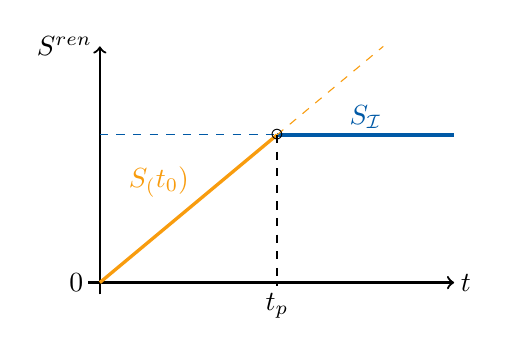
\begin{tikzpicture}[scale=0.75]
\draw[->,thick] (0,-0.2) to (0,4);
\draw[->,thick] (-0.2,0) to (6,0);

\node at (-0.6,4) {$S^{\text{ren}}$};
\node at (6.2,0) {$t$};

\draw[-,blue!30!teal,very thick] (3,2.5) to (6,2.5);
\draw[-,dashed,blue!30!teal] (0,2.5) to (3,2.5);

\draw[-,dashed,yellow!20!orange] (3,2.5) to (4.8,4);
\draw[-,yellow!20!orange,very thick] (0,0) to (3,2.5);
\node at (3,2.5) {$\circ$};
\draw[-,dashed] (3,2.5) to (3,0);
\draw[-] (3,0) to (3,-0.05);
\node at (3,-0.4) {$t_p$};


\node[yellow!20!orange] at (1,1.7) {$S_\varnothing(t_0)$};
\node[blue!30!teal] at (4.5,2.8) {$S_{\mathcal{I}}$};

\node at (-0.4,0) {$0$};
\end{tikzpicture}
\caption{On the left is the two-sided thermal configuration of (II) featuring both the $t = t_0$ radiation region $\mathcal{R}^L(t_0) \cup \mathcal{R}^R(t_0)$ and the island $\mathcal{I}$ which emerges at late times. The right figure is a sketch of the (eternal) Page curve depicting (renormalized) entanglement entropy versus time---initially the time-dependent no-island entropy $S_\varnothing$ is minimal, but it eventually exceeds the non-trivial island entropy $S_{\mathcal{I}}$. This curve can be obtained by computing (renormalized) areas in the (III) configuration.}
\label{figs:eternalBH}
\end{figure}